\section{Problem Statement}%
\label{sec:problem_statement}

\subsection{Toroidal Graph}%
\label{sub:toroidal_graph}


According to \href{http://azspcs.com/Contest/Nearness}{AZSPCS}, a toroidal graph is defined as an $N\times N$ grid of unique tokens -- here presented as $IJ$, where $I$ and $J$ represent the alphabetic indices (eg. $A$ corresponds to 1) of the rows and columns respectively -- whose edges wrap around. For $N=4$, the grid is shown in \autoref{fig:toroidExample}. The tokens outside of the square grid represent tokens which ``wrap around'' the grid (hence the toroidal grid).
\begin{figure}[htpb]
    \centering
    \toroidWarp{4}
    \caption{A $4\times 4$ toroidal grid}%
    \label{fig:toroidExample}
\end{figure}

\subsection{Evaluation Function}%
\label{sub:evaluation_function}

The goal of the challenge (and hence this essay) is to create a new grid -- with tokens from the original grid to be arranged in any order -- which minimizes a loss function (which quantifies failure) defined as follows:
\begin{enumerate}
    \item For each pair of tokens, calculate the squared distance between them in the new grid,
\item multiply it with its squared distance within the original grid
\item The sum of these multiplications is the value of the loss
\end{enumerate}
As is with all loss functions, the goal is to minimize the loss function.

\subsubsection{Distance Metric}%
\label{ssub:distance_metric}
If 2 two-dimensional coordinates are defined as $s_1=(x_1,y_1)$ and $s_2=(x_2,y_2)$, the Euclidean distance $d$ is defined as

\begin{equation}
    \label{eq:euclid}
    d(s_1,s_2)=\sqrt{(x_2-x_1)^2+(y_2-y_1)^2}=\sqrt{(\Delta x)^2+(\Delta y)^2}
\end{equation}

and the squared Euclidean distance $d^2$ evaluates to
\begin{equation}
    d^2(s_1,s_2)=(\Delta x)^2+(\Delta y)^2
    \label{eq:squaredEuclid}
\end{equation}
simplifying much of the computation.

But with a toroidal surface, both $\Delta x$ and $\Delta y$ have 2 possible values. A one-dimensional case with toroidal surface of length $N$ is shown in \autoref{fig:2distanceexample}. These two distances can be written as
\begin{align*}
    %\label{eq:naiveToroidDistance}
    \Delta_1(x)&=x_2-x_1 \\
    \Delta_2(x)&=(x_1-0)+(N-x_2)=x_1+N-x_2
\end{align*}

\begin{figure}[tpb]
    \centering
    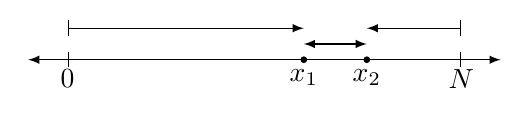
\begin{tikzpicture}
        \draw[latex-latex] (-3,0) -- (3,0);
        \draw[|-|] (-2.5,0) node[below] {$0$} -- (2.5,0) node[below] {$N$};
        %\draw[|-|] (-2.5,-0.5) -- node[below] {$N$} (2.5,-0.5);
        \filldraw (0.5,0) circle (1pt) node[below] {$x_1$};
        \filldraw (1.3,0) circle (1pt) node[below] {$x_2$};
        \draw[latex-latex] (0.5,0.2) -- (1.3,0.2);
        \draw[latex-|] (1.3,0.4) -- (2.5,0.4);
        \draw[|-latex] (-2.5,0.4) -- (0.5,0.4);
    \end{tikzpicture}
    \caption{One-dimensional diagram of toroidal distance}%
    \label{fig:2distanceexample}
\end{figure}


To obtain a general equation which works with both $x_1>x_2$ and $x_1<x_2$, we can write
\begin{align*}
    \Delta_1(x)&=\lvert x_2-x_1 \rvert \\
    \Delta_2(x)&=\min{(x_1,x_2)}+N-\max{(x_1,x_2)}
    %\label{eq:absoluteToroidDistance}
\end{align*}
where $\lvert a\rvert$ is the absolute value of $a$, $\min{(a,b)}$ and $\max{(a,b)}$ are defined as the minimum and maximum of $a$ and $b$ respectively. $\min$ and $\max$ are used to determine the  ``left-most'' and the ``right-most'' numbers.

Since, the distance can only have 1 value, it is defined as
\begin{align*}
    \Delta x=\min{(\Delta_1(x),\Delta_2(x))}
\end{align*}

Generalizing it to 2 dimensions, we get
\begin{align*}
    d(s_1,s_2)&=\sqrt{(\Delta x)^2+(\Delta y)^2} \\
    d^2(s_1,s_2)&=(\Delta x)^2+(\Delta y)^2
\end{align*}
where $d^2$ is the distance metric to be used in our calculations.

\subsubsection{Token Comparisons}%
\label{ssub:token_comparisons}
To be able to perform comparisons for every possible pair of tokens, a grid of comparisons (between two tokens to obtain distances) is required. A viable approach would be to to represent the comparison in a 4-dimensional grid (or tensor), where for every token in the toroidal grid, we compare it to every token. An example of the structure of the comparison for a $2\times 2$ grid is shown in \autoref{fig:4dcomparison}. The white boxes denote duplicate comparisons (eg. $
\begin{smallmatrix}
    BA\\ AA
\end{smallmatrix}
$ is identical to
$
\begin{smallmatrix}
    AA\\ BA
\end{smallmatrix}
$), because the distance is invariant to the order of the tokens.


But since removing the irregularly shaped duplicate entries will be a hassle, we can simplify the problem by reducing the dimensionality of the grid: from a 4-dimensional grid $A_{ijkl}$ into a 2-dimensional grid $A_{ij,kl}$. An example is shown in \autoref{fig:2dcomparison}. By doing so, we can easily remove the duplicate entries by multiplying it with the upper triangular matrix, see \autoref{ssub:loss_function_as_matrix_multiplications}. Let $C(X)$ denote a function mapping, returning this comparison grid for an input toroidal grid $X$. Note that if $X$ is a grid of the form $N\times N$, $C(X)$ has the form $N^2\times N^2$

\begin{figure}[htpb]
    \centering
    \label{fig:twodcomparisonGrid}
\end{figure}

\begin{figure}[htpb]
    \centering
    \begin{subfigure}[t]{0.5\textwidth}
    \begin{center}
    \nestedToroid{2}
    \end{center}
    \caption{$A_{ijkl}$, a 4-dimensional comparison}
    \label{fig:4dcomparison}
    \end{subfigure}%
    ~
    \begin{subfigure}[t]{0.5\textwidth}
    \begin{center}
    \twodcomparison{2}
    \end{center}
    \caption{$A_{ij,kl}$ a 2-dimensional comparison}
    \label{fig:2dcomparison}
    \end{subfigure}

    \caption{Tensors $C$ representing comparison grids of a $2\times 2$ toroidal grid, where every element represents the toroidal distance between $T_{ij}$ and $T_{kl}$, where $T$ is the toroidal grid. Shaded cells denote unique comparisons.}%
    \label{fig:comparisonGrids}
\end{figure}

\subsubsection{Loss Function as Matrix Multiplications}%
\label{ssub:loss_function_as_matrix_multiplications}
Let $\odot$ denote the element-wise matrix multiplication, and $O$ denotes the original grid. The loss function for toroidal grid $X$ is equal to
\begin{equation}
    L(x)=\sum C(X)\odot C(O)\odot U
\end{equation}
where $C(X),C(O),U$ are matrices of the form $N^2\times N^2$, and $U_{ij}$ is defined with the piece-wise defined function:
\begin{equation}
    U_{ij}=
    \begin{cases}
        1, & j\geq i \\
        0, & j<i
    \end{cases}
\end{equation}
an example the matrix U with shape $4\times 4$ is as follows:
 \begin{equation}
    \begin{pmatrix}
        1&1&1&1\\
        0&1&1&1\\
        0&0&1&1\\
        0&0&0&1
    \end{pmatrix}
\end{equation}
